\documentclass[journal, a4paper]{IEEEtran}

\usepackage{cite}
\usepackage{graphicx}
\usepackage{psfrag} 
\usepackage{subfigure}
\usepackage{url}
\usepackage{stfloats} 
\usepackage{amsmath}
\usepackage{colortbl}
\usepackage{xcolor}
\usepackage{tikz}
\usepackage{pgfplots}
\interdisplaylinepenalty=2500
\usepackage{array}
\usepackage{tabularx}
\usetikzlibrary{shapes}

\setlength{\parskip}{\baselineskip}%
\setlength{\parindent}{0pt}%

\begin{document}

\title{NLP Project: Authorship Detection of Twitter Tweets}
\author{Clemens Biehl, Daniel Wehner, Fabian Otto, Philipp Kapelle
\thanks{TU Darmstadt, WS 2017/2018.}}
\markboth{Natural Language Processing and the Web}{}
\maketitle

\begin{abstract}
In our project we worked on the authorship detection of Twitter tweets. This report gives a short summary of the results which we could produce during the project.
\end{abstract}
	
\section{Introduction and Research Problem}
Millions of texts and posts are published on social media platforms such as Twitter or Facebook every day. The identification of the authorship is often a crucial task in Natural Language Processing. This might be helpful when checking the authenticity of a post. In this project we therefore aim to classify Twitter Tweets to identify the authors of the tweets and try to answer the following questions:

\begin{itemize}
\item Which types of writing-style features are effective for identifying the authorship of online messages? For that we tried various combinations of features and evaluated those combinations.
\item Which classifiers perform best for identifying the authorship of online messages?
\item To what extent can authorship-identification techniques be applied to online messages with different numbers of authors and messages?
\end{itemize}

\section{Data Provisioning}
\label{sec:provisioning}

As already mentioned, Twitter will be the source for the data to be analyzed. We focused on tweets of 20 famous politicians of the English-speaking world since we confined ourselves to english tweets. We collected tweets from the following accounts:

\footnotesize
\textit{
realDonaldTrump, BarackObama, ChuckGrassley, RepJaredPolis, BorisJohnson, clairecmc, ChrisChristie, jahimes, jeremycorbyn, CarolineLucas, David\_Cameron, BernieSanders, RonPaul, SpeakerRyan, mike\_pence, DavidLammy, timfarron, Ed\_Miliband, ChukaUmunna, tom\_watson
}
\normalsize

The number of tweets collected per account is 1,000, which makes 20,000 tweets in total. When guessing the authors randomly, we would get an accuracy of approximaltey 5\,\% (since the training data consists of tweets from 20 different authors). This is our baseline. We should have an accuracy better than 5\,\%.

\begin{figure}
\caption{JSON representation of a tweet written by Barack Obama that was crawled from Twitter}
\footnotesize
\begin{verbatim}
{  
   "in_reply_to_status_id_str":null,
   "in_reply_to_status_id":null,
   "coordinates":null,
   "created_at":"Mon Jan 15 14:46:02 +0000 2018",
   "truncated":false,
   "in_reply_to_user_id_str":null,
   "source":"<a href=\"http://twitter.com/download/
     iphone\" rel=\"nofollow\">Twitter for
     iPhone<\/a>",
   "retweet_count":367963,
   "retweeted":false,
   "geo":null,
   "in_reply_to_screen_name":null,
   "is_quote_status":false,
   "entities":{  
      "urls":[  

      ],
      "hashtags":[  

      ],
      "user_mentions":[  

      ],
      "symbols":[  

      ]
   },
   "full_text":"Dr. King was 26 when the Montgomery
      bus boycott began. He started small, rallying
      others who believed their efforts mattered,
      pressing on through challenges and
      doubts to change our world (...)",
   "id_str":"952914779458424832",
   "in_reply_to_user_id":null,
   "display_text_range":[  
      0,
      279
   ],
   "favorite_count":1393878,
   "id":952914779458424832,
   "place":null,
   "contributors":null,
   "lang":"en",
   "user":{  
      "id_str":"813286",
      "id":813286
   },
   "favorited":false
}
\end{verbatim}
\normalsize
\end{figure}

\section{Pipeline}
\label{sec:pipeline}

\begin{figure}[h]
	\caption{Visualization of the pipeline built for the authorship identification. After providing the data by the crawler, the data is
	 preprocessed. The feature extraction phase takes care of creating useful features for classification for the training of the model.
	The last step is the evaluation of the model.}
	\vspace*{5mm}
	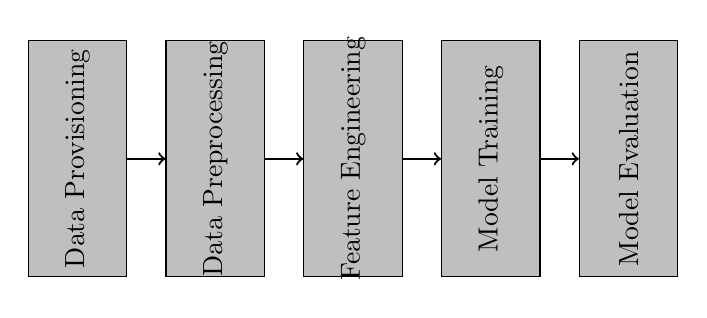
\begin{tikzpicture}
		\node[rectangle,fill=lightgray,draw=black,minimum height=3cm, minimum width=1.25cm] (A) at (0,0) {};
		\node[rectangle,fill=lightgray,draw=black,minimum height=3cm, minimum width=1.25cm] (B) at (1.75,0) {};
		\node[rectangle,fill=lightgray,draw=black,minimum height=3cm, minimum width=1.25cm] (C) at (3.5,0) {};
		\node[rectangle,fill=lightgray,draw=black,minimum height=3cm, minimum width=1.25cm] (D) at (5.25,0) {};
		\node[rectangle,fill=lightgray,draw=black,minimum height=3cm, minimum width=1.25cm] (E) at (7,0) {};

		\draw[thick,->] (A) -- (B);
		\draw[thick,->] (B) -- (C);
		\draw[thick,->] (C) -- (D);
		\draw[thick,->] (D) -- (E);

		\node[rotate=90] at (0,0) {Data Provisioning};
		\node[rotate=90] at (1.75,0) {Data Preprocessing};
		\node[rotate=90] at (3.5,0) {Feature Engineering};
		\node[rotate=90] at (5.25,0) {Model Training};
		\node[rotate=90] at (7,0) {Model Evaluation};
	\end{tikzpicture}
\end{figure}

\textbf{Data Provisioning}: For information see section \ref{sec:provisioning}

\textbf{Feature Engineering}: Please see section \ref{sec:features}

\textbf{Model Training and Evaluation}: Please refer to section \ref{sec:training-eval} 

\section{Feature Engineering}
\label{sec:features}

The feature engineering phase is crucial for the success of the project since the performance of the classifiers depends significantly on the quality of the features used. Table \ref{tab:features} summarizes the features which we have taken into account when training the classifiers.  

\begin{table}[!hbt]
	\begin{center}
		\caption{List of features which were considered for training the classifiers.}
		\label{tab:features}
		\begin{tabularx}{80mm}{| l | X |}
			\hline
			\rowcolor{lightgray}
			\textbf{Feature}			& \textbf{Explanation}						\\ \hline\hline
			Total number of chars		& How long is the tweet						\\ \hline
			Emoticon ratio		  	& Proportion of emoticons in the text. 			\\ \hline
			Number of hashtags		& How many hashtags are used in the tweet. 	\\ \hline
			Word frequencies        	& Which words are used frequently 				\\ \hline
			Lexical diversity			& How rich is the vocabulary of the author? 		\\ \hline
			Contextuality Measure		& Score between 0 and 100
								  	(0 very context dependent = many pronouns, adverbs, ...;
									100 not content dependent = many nouns, ...) 
																				\\ \hline
			Exclamation Ratio			& How many exclamation marks are used?		\\ \hline
			Superlative Ratio			& Proportion of superlatives in the tweet?		\\ \hline
			PastVsFuture				& Ratio of verbs in past tense/present tense		\\ \hline
			\hline
		\end{tabularx}
	\end{center}
\end{table}

With emoticons playing a central role in social media they represent a good feature to consider. Therefore, the emoticon ratio (ER) is calculated (the number of tokens which represent emoticons divided by the total number of tokens in the text).

Other features like sentence features did not perform well since twitter texts are very short.

\begin{equation}
	\text{ER} = \frac{\text{\# of emoticon tokens}}{\text{\# of tokens}}
\end{equation}

Also very characteristic for specific authors is the number of hashtags they use when writing a tweet, the word frequencies (does the author prefer specific words over other words) and the lexical diversity (also known as type-token ratio [TTR] which analyzes how many different words are used in the tweet)

\begin{equation}
\text{TTR} = \frac{V(N)}{N}
\end{equation}

Other measures for lexical diversity/vocabulary richness:

\begin{equation}
\text{Yule's $K$} = C \left[ -\frac{1}{N} + \sum_{m=1}^{m_{max}} V(m,N)\left(\frac{m}{N}\right)^2 \right]
\end{equation}

\begin{equation}
\text{Simpson's $D$} = \sum_{m=1}^{m_{max}} V(m,N)\frac{m}{N}\frac{m-1}{N-1}
\end{equation}

\begin{equation}
\text{Herdan $V_m$} = \sqrt{\sum_{m=1}^{m_{max}}V(m,N)\left(\frac{m}{N}\right)^2-\frac{1}{V(N)}} 
\end{equation}

\begin{equation}
\text{Sichel's $S$} = \frac{V(1,N)}{V(N)}
\end{equation}

\begin{equation}
\text{Honores $R$} = 100 \frac{\log \left(N\right)}{1 - \frac{V(1,N)}{V(N)}}
\end{equation}

\begin{equation}
\text{Brunet's $W$} = N^{V - c} \quad \text{usually $c = 0.17$}
\end{equation}

\begin{equation}
\text{Uber Index} = \frac{\log\left(N\right)^2}{\log \left(N\right) - \log \left(V(N)\right)}
\end{equation}

\begin{tabular}{@{}>{$}l<{$}l@{}}
	N	 		& Length of text \\ 
 	V(N) 		& Size of vocabulary \\
    	V(m,N) 		& Number of words in $N$ occuring $m$ times \\
	V(1,N) 		& Number of \textbf{Hapax Legomena} \\
	V(2,N) 		& Number of \textbf{Hapax Dislegomena} \\
    	m_{max}	& maximal frequency
\end{tabular}

Another feature of interest is the contextuality measure which indicates how context-dependent a text is. The contextuality measure produces values between 0 and 100. A value of 0 indicates a very context-dependent text which contains many pronouns, adverbs, etc. The higher the value the less context-dependent the text is (the text is then said to be \textit{formal} as opposed to \textit{contextual}). This is the formula which computes the score:

\begin{equation}
F = \frac{n + a + p + d - pr - v - ad - if + 100}{2}
\end{equation}

\begin{tabular}{@{}>{$}l<{$}l@{}}
    n 		& noun frequency \\
    a 		& adjective frequency \\
    p 		& preposition frequency \\
    d 		& determiner frequency \\
    pr		& pronoun frequency \\
    v			& verb frequency \\
    ad		& adverb frequency \\
    if			& interjection frequency \\	
\end{tabular}

\section{Evaluation}
\label{sec:training-eval}

As a basis we used the \texttt{WekaTwitterSentimentDemo} which we found in the DKPro\,TC GitHub Repository which resulted in an accuracy of approximately 9\,\% (Used features in the demo: EmoticonRate and Number of Hashtags, Number of Tokens per Sentence). We used this as the baseline and added further features. The results which could be generated are summarized in table \ref{tab:results} and in figure \ref{fig:results} respectively.

\begin{table}[!hbt]
	\begin{center}
		\caption{Evaluation results for different feature setups ordered by increasing accuracy. Classifier = \textbf{Naive Bayes}}
		\label{tab:results-nb}
		\begin{tabularx}{80mm}{| l | X | r |}
			\hline
			\rowcolor{lightgray}
			\multicolumn{3}{| c |}{\textbf{Naive Bayes}} 									\\ \hline
			\rowcolor{lightgray}
			\textbf{Nr.}		&	\textbf{Setup}					& \textbf{Accuracy}		\\ \hline\hline
			1			&	\texttt{WekaTwitterSentimentDemo}	& \textbf{9.00\,\%}		\\ \hline
			2			&	TTR 	(Type-Token-Ratio)			& \textbf{15.49\,\%}		\\ \hline
			3			&	TTR + Contextuality Measure			& \textbf{19.49\,\%}		\\ \hline
			4			&	TTR + UpperCase + Alphabetic + Digits + WhiteSpaces + TabSpaces
																& \textbf{20.23\,\%}		\\ \hline
			5			& 	TTR + Contextuality Measure + Exclamation Ratio
																& \textbf{22.45\,\%}		\\ \hline
			6			&	TTR + Contextuality Measure + Exclamation Ratio + Superlative Ratio + PastVsFuture 
																& \textbf{24.00\,\%}		\\ \hline
			7			&	TTR + Contextuality Measure + Exclamation Ratio + Superlative Ratio 
																& \textbf{25.32\,\%}		\\ \hline
			8			&	TTR + Contextuality Measure + Exclamation Ratio + Superlative Ratio +
							Nr of Tokens + Character Features + N-Grams
																& \textbf{42.40\,\%}		\\ \hline
			9			&	TTR + Contextuality Measure + Exclamation Ratio + Superlative Ratio +
							Nr of Tokens + Character Features + N-Grams + POS-NGrams
																& \textbf{44.31\,\%}		\\ \hline
			\hline
		\end{tabularx}
	\end{center}
\end{table}

% Bar diagram which visualizes the results of the different setups
\begin{figure}[!hbt]
	\begin{center}
		\caption{Evaluation results for different feature/classifier setups ordered by increasing accuracy}
		\label{fig:results}
		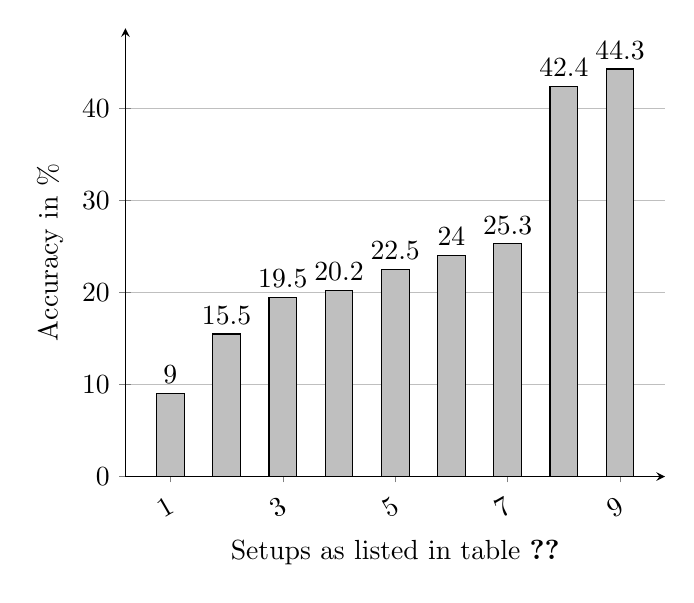
\begin{tikzpicture}
			\begin{axis}[
    				ybar, bar width=10pt,
				nodes near coords, nodes near coords align=above, point meta=rawy,
 				axis x line=bottom, axis y line=left, ymajorgrids=true,
				ylabel=$\mathrm{Accuracy\ in\ \%}$, ymin=0, ytick={0,10,20,30,40,50,60,70,80,90,100},
				enlargelimits=auto,
    				xlabel=Setups as listed in table \ref{tab:results-nb}, symbolic x coords={1,2,3,4,5,6,7,8,9},
    				x tick label style={rotate=30,anchor=north east},
    			]

    				\addplot[fill=lightgray] coordinates {
      					(1,9.0)
      					(2,15.5)
					(3,19.5)
					(4,20.2)
					(5,22.5)
					(6,24.0)
					(7,25.3)
					(8,42.4)
					(9,44.3)
    				};
  			\end{axis} 
		\end{tikzpicture}
	\end{center}
\end{figure}

\begin{table}[!hbt]
	\begin{center}
		\caption{Evaluation results for different feature setups ordered by increasing accuracy.
		Classifier = \textbf{Random Forests}}
		\label{tab:results-rf}
		\begin{tabularx}{80mm}{| l | X | r |}
			\hline
			\rowcolor{lightgray}
			\multicolumn{3}{| c |}{\textbf{Random Forest}} 								\\ \hline
			\rowcolor{lightgray}
			\textbf{Nr.}		&	\textbf{Setup}					& \textbf{Accuracy}		\\ \hline\hline
			1			&	\texttt{WekaTwitterSentimentDemo}	& \textbf{9.35\,\%}		\\ \hline
			2			&	TTR (Type-Token-Ratio)				& \textbf{17.59\,\%}		\\ \hline
			3			&	TTR + Contextuality Measure			& \textbf{97.30\,\%}		\\ \hline
			4			&	TTR + UpperCase + Alphabetic + Digits + WhiteSpaces + TabSpaces
																& \textbf{0.00\,\%}		\\ \hline
			5			& 	TTR + Contextuality Measure + Exclamation Ratio
																& \textbf{0.00\,\%}		\\ \hline
			6			&	TTR + Contextuality Measure + Exclamation Ratio + Superlative Ratio + PastVsFuture 
																& \textbf{0.00\,\%}		\\ \hline
			7			&	TTR + Contextuality Measure + Exclamation Ratio + Superlative Ratio 
																& \textbf{0.00\,\%}		\\ \hline
			\hline
		\end{tabularx}
	\end{center}
\end{table}

% Bar diagram which visualizes the results of the different setups
\begin{figure}[!hbt]
	\begin{center}
		\caption{Evaluation results for different feature/classifier setups ordered by increasing accuracy}
		\label{fig:results}
		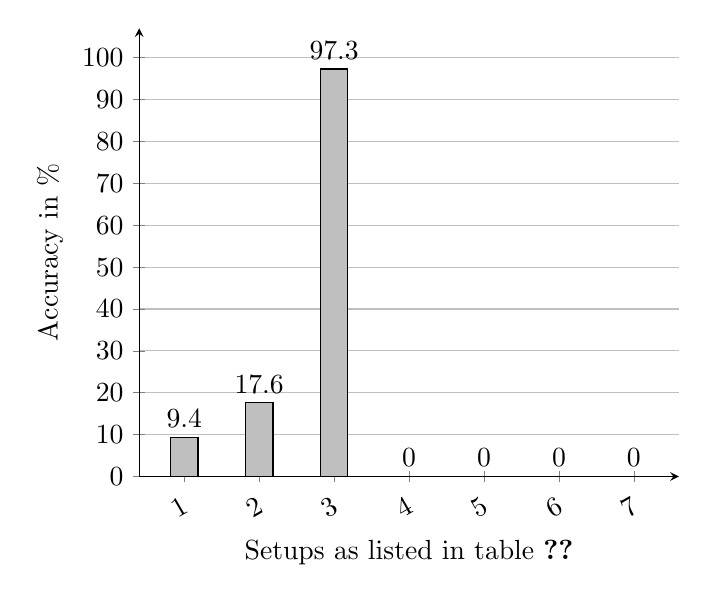
\begin{tikzpicture}
			\begin{axis}[
    				ybar, bar width=10pt,
				nodes near coords, nodes near coords align=above, point meta=rawy,
 				axis x line=bottom, axis y line=left, ymajorgrids=true,
				ylabel=$\mathrm{Accuracy\ in\ \%}$, ymin=0, ytick={0,10,20,30,40,50,60,70,80,90,100},
				enlargelimits=auto,
    				xlabel=Setups as listed in table \ref{tab:results-rf}, symbolic x coords={1,2,3,4,5,6,7},
    				x tick label style={rotate=30,anchor=north east},
    			]

    				\addplot[fill=lightgray] coordinates {
      					(1,9.4)
      					(2,17.6)
					(3,97.3)
					(4,0.00)
					(5,0.00)
					(6,0.00)
					(7,0.00)
    				};
  			\end{axis} 
		\end{tikzpicture}
	\end{center}
\end{figure}

\section{Deep Learning}

Extracting the features is very tedious and it is more or less a trial and error process. There are many combinations of features that have to be taken into account and which have to be evaluated. A remedy for that is for example a \textbf{Deep Learning} approach. Such approaches have become very famous recently and also for Natural Language Processing there are several application areas for such methods. Deep Learning is capable of automating this combersome process by making use of several layers that are responsible for feature extraction and transformation. The results of one layer represent the input of the next layers. Very often \textbf{Artificial Neural Networks (ANN)} are used in such cases.

\begin{figure}[h]
	\caption{A simple neural network}
	\centering
	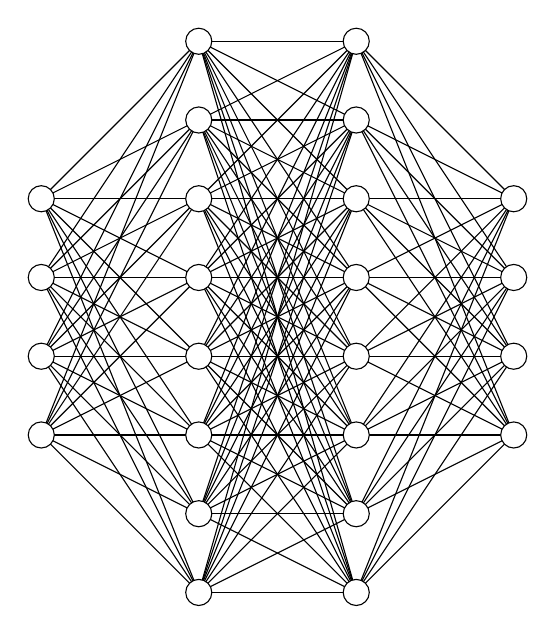
\begin{tikzpicture}
		\foreach \y in {1, 2, 3, 4, 5, 6, 7, 8}{
			\draw (0,3) -- (2,\y);
			\draw (0,4) -- (2,\y);
			\draw (0,5) -- (2,\y);
			\draw (0,6) -- (2,\y);
		}

		\foreach \y in {1, 2, 3, 4, 5, 6, 7, 8}{
			\draw (2,1) -- (4,\y);
			\draw (2,2) -- (4,\y);
			\draw (2,3) -- (4,\y);
			\draw (2,4) -- (4,\y);
			\draw (2,5) -- (4,\y);
			\draw (2,6) -- (4,\y);
			\draw (2,7) -- (4,\y);
			\draw (2,8) -- (4,\y);
		}
		
		\foreach \y in {1, 2, 3, 4, 5, 6, 7, 8}{
			\draw (4,\y) -- (6,3);
			\draw (4,\y) -- (6,4);
			\draw (4,\y) -- (6,5);
			\draw (4,\y) -- (6,6);
		}

		\foreach \y in {3, 4, 5, 6}
			\node[circle,draw=black,fill=white] at (0,\y) {};
		\foreach \y in {1, 2, 3, 4, 5, 6, 7, 8}
			\node[circle,draw=black,fill=white] at (2,\y) {};
		\foreach \y in {1, 2, 3, 4, 5, 6, 7, 8}
			\node[circle,draw=black,fill=white] at (4,\y) {};
		\foreach \y in {3, 4, 5, 6}
			\node[circle,draw=black,fill=white] at (6,\y) {};
	\end{tikzpicture}
\end{figure}

\section{Component Diagram}

\section{Conclusion}
This section summarizes the paper.

\begin{thebibliography}{2}

	\bibitem{Zheng06}
	Zheng, Rong and Li, Jiexun and Chen, Hsinchun and Huang, Zan. A Framework for Authorship Identification
	of Online Messages: Writing-Style Features and Classification Techniques. {\em Journal of the American
	Society for Information Science and Technology},
	vol.~57, no.~3, pp.~378-393, 2006.

	\bibitem{Hout07}
	Hout, Roeland and Vermeer, Anne. Comparing measures of lexical richness. {\em Modelling and assessing vocabulary 
	knowledge}, pp.~93-116, 2007.

	\bibitem{Fissette10}
	Fissette, Marcia. Author identification in short texts. 2010.

	\bibitem{Green13}
	Green, Rachel M. and Sheppard, John W. Comparing Frequency- and Style-Based Features for Twitter
	Author Identification. {\em AAAI Press}, 2013.
	
	\bibitem{Heylighen02}
	Heylighen, Francis; Dewaele, Jean-Marc. Variation in the Contextuality of Language: An Empirical Measure.
	{\em Foundations of Science}, vol.~7, no.~3, pp.~293-340, September 2002.

	\bibitem{Aihara15}
	Tanaka-Ishii, Kumiko and Aihara, Shunsuke. Computational Constancy Measures of Texts—Yule's K and Rényi's Entropy.
	{\em Computational Linguistics} vol.~41, no.~3, pp.~481-502, September 2015.

	\bibitem{Tweedie98}
	Tweedie, Fiona J. and BaayenHow, R. Harald. Variable May a Constant be? Measures of Lexical Richness in Perspective.
	{\em Computers and the Humanities} vol.~32, no.~5, pp.~323-352, September 1998.	

	\bibitem{Bhatia}
	Bhatia Archna et al. TweetNLP, Carnegie Mellon. \url{http://www.cs.cmu.edu/~ark/TweetNLP}

\end{thebibliography}

\end{document}